\section*{Question 9}
\fakesection{9}

This problem repeats the single-rate filtering of Question 1 using Simulink. Figure \ref{fig:q9_simulink} presents the Simulink model, where \texttt{num(z)} is the coefficients of the filter designed in Question 1.

\begin{figure}[ht]
    \centering
    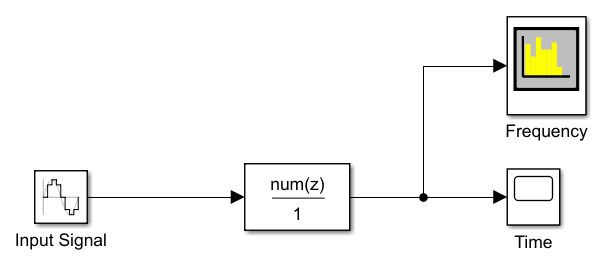
\includegraphics[width=0.55\textwidth]{images/q9_simulink.png}
    \caption{Simulink model for single-rate filtering}
    \label{fig:q9_simulink}
\end{figure}

Figure \ref{fig:q9_inpt} shows the input signal (with \texttt{num(z)} as \texttt{[1]}) in the time and frequency domains.

\begin{figure}[ht]
    \centering
    \begin{subfigure}[b]{0.69\textwidth}
        \centering
        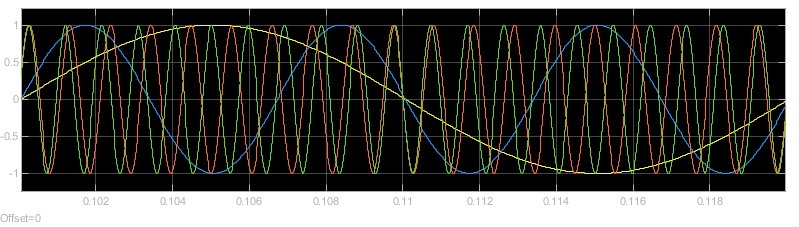
\includegraphics[width=\textwidth]{images/q9_inpt_time.png}
    \end{subfigure}
    \\
    \begin{subfigure}[b]{0.7\textwidth}
        \centering
        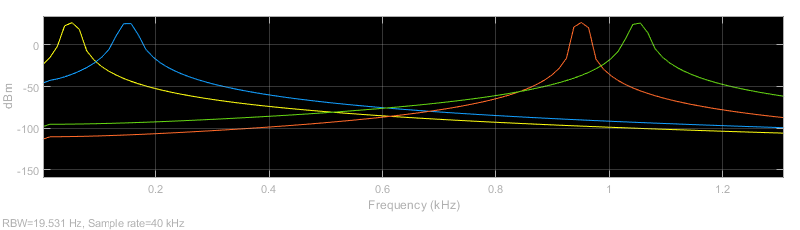
\includegraphics[width=\textwidth]{images/q9_inpt_freq.png}
    \end{subfigure}
    \caption{Input signal contains tones at 50, 150, 950 and 1050 Hz}
    \label{fig:q9_inpt}
\end{figure}

Figure \ref{fig:q9_filt} shows the signal after applying the Kaiser-windowed LPF designed in Question 1.

\begin{figure}[ht!]
    \centering
    \begin{subfigure}[b]{0.69\textwidth}
        \centering
        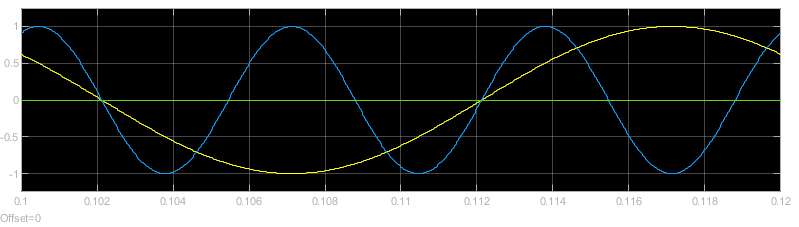
\includegraphics[width=\textwidth]{images/q9_filt_time.png}
    \end{subfigure}
    \\
    \begin{subfigure}[b]{0.7\textwidth}
        \centering
        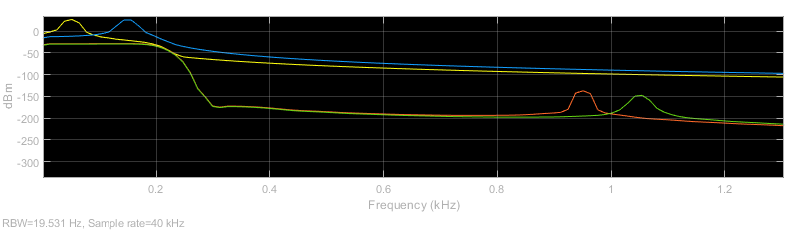
\includegraphics[width=\textwidth]{images/q9_filt_freq.png}
    \end{subfigure}
    \caption{Filtered signal containing only tones at 50 and 150 Hz}
    \label{fig:q9_filt}
\end{figure}

The higher tones are visibly and audibly attenuated; hence, the filtering is successful.
